
\documentclass{beamer}
\usetheme{boxes}

\usepackage{tikz}

\begin{document}

\begin{frame}
\begin{center}
\begin{tikzpicture}
\def\shift{1cm}
\tikzset{
  every node/.style={minimum width=\shift, minimum
  height=\shift,font=\Large},
  every path/.style={->,draw},
  reg/.style={draw},
  idx/.style={blue,font=\it},
  current/.style={thick},
  j/.style={current, red, draw},
  i/.style={green!40!black},
  dummy/.style={brown!50!black}
}

\foreach \i/\n in {0/55,1/33,2/77,3/22,4/88,5/44,6/66} {
    \node[reg] (reg\i) at (\i*\shift,0) {\n};
    \node[idx] (idx\i) [above of=reg\i] {\i};
}
\node<2-9,11->[reg,dummy] (regN) at (7*\shift,0) {\only<1-9>{44}\only<11->{99}};
\node<2-9,11->[idx,dummy] (idxN) [above of=regN] {7};
\node<2,11>[text width=2cm,dummy] [above of=idxN,yshift=.5*\shift] {\small registro fict\'icio};

\node [above of=reg0,yshift=2.5*\shift] {\tt buscaQ(\only<1-9>{44}\only<10->{{\color{red}99}});};

\foreach \j/\f in {0/3, 1/4, 2/5, 3/6, 4/7, 5/8} {
         \node<\f>[i] (I\f) [above of=reg\j, yshift=1.5*\shift] {\tt i};
         \path<\f> (idx\j) -- (I\f);
         \node<\f>[circle,blue,draw] at (reg\j) {};
         \node<\f> (key searched\j) [below of=reg\j, yshift=-\shift] {44};
         \path<\f> (reg\j) -- node [right] {$=?$} (key searched\j);
}

\node<9>[red, circle, thick, draw] (found) at (5*\shift,0) {};
\node<9>[red] (idx found) [below of=found,yshift=-\shift] {5};
\node<9>[red,circle,dotted, thick, draw]  at (idx5) {};
\path<9> (found) -- (idx found) node[left] {\scriptsize retorna\ \ };

\foreach \j/\f in {0/12, 1/13, 2/14, 3/15, 4/16, 5/17, 6/18, N/19} {
         \node<\f>[i] (I\f) [above of=reg\j, yshift=1.5*\shift] {\tt i};
         \path<\f> (idx\j) -- (I\f);
         \node<\f>[circle,blue,draw] at (reg\j) {};
         \node<\f> (key searched\j) [below of=reg\j, yshift=-\shift] {\color{red}99};
         \path<\f> (reg\j) -- node [right] {$=?$} (key searched\j);
}

\node<20>[red] (idx notfound) [below of=regN,yshift=-\shift] {\bf -1};
\path<20> (regN) -- node[right] {$i=N$} (idx notfound) node[left] {\scriptsize retorna\ \
\ } ;


\end{tikzpicture}

\end{center}
\end{frame}


\end{document}

